\fxnote{Konsitens i forhold til vinklen, 90 grader. Tegning med tape på væggen - vinkelmåler. Ny måle metode.}
\section{Pilotforsøg}
I dette bilag beskrives pilotforsøgets fremgangsmåde samt, hvilke resultater, der opsamles. 

\subsection{Formål}
Dette pilotforsøg har til formål at kunne præcisere samt optimere kravspecifikationerne i de enkelte blokke, hvorved uklare parametre forventes besvaret. Disse parametre omfatter identificering af støjsignaler samt EMG-signalets frekvensområde. Parametrene vil forsøges besvaret ud fra målinger ved udførelse af en squat-øvelse.
Hertil anvendes elektroder og to accelerometre som sensorer. På baggrund af dette opstilles følgende formål:  

\subsubsection{EMG-måling}
\begin{enumerate}
\item Opsamling af signal fra rectus femoris og biceps femoris
\begin{itemize}
\item Sammenligning af muskelaktivitet oprejst og i en squat-øvelse 
\end{itemize}
\item Identificering af støjsignaler
\item Identificering af frekvensområde
\item Identificering af gain til mikroprocesserens operationsspænding \fxnote{Finde operationsspænding og angiv den her}
\end{enumerate}

\subsubsection{Accelerometre}
\begin{enumerate}
\item Identificering af knæleddets vinkel
\end{enumerate}

\subsection{Materialer} 
\begin{itemize}
\item To EMG-forstærkere
\item Elektroder \fxnote{hvad for nogle elektroder snakker vi om, husk}
\item Desinfektionsservietter
\item Skraber
\item To accelerometre ADXL335Z
\item Tape
\item Breadboards
\item Computer med MATLAB
\item CY8CKIT-042-BLE \fxnote{Opmærksom - er dette den eneste komponent?}
\end{itemize}

\subsection{Metode}
Til forsøget benyttes to EMG-forstærkere. Dette giver to sæt elektroder til differensmåling af henholdsvis rectus femoris og biceps femoris. Hvert sæt elektroder består af én positiv-, negativ- samt én referenceelektrode. 
For at identificere elektrodeplacering på musklerne tages der udgangspunkt i Seniam's anvisning for elektrodeplacering \citep{seniam2016}. 
Elektoderne placeres midt for linjen mellem ischial tuberosity og den laterale epifyse af tibia ved måling over biceps femoris. Ved måling af rectus femoris placeres elektroderne midt for linjen mellem anterior spina iliaca superior og den superior del af patella \citep{seniam2016}. Placeringen af elektroderne illustreres af \autoref{fig:laarmuskler}. 

\begin{figure}[H]
\centering
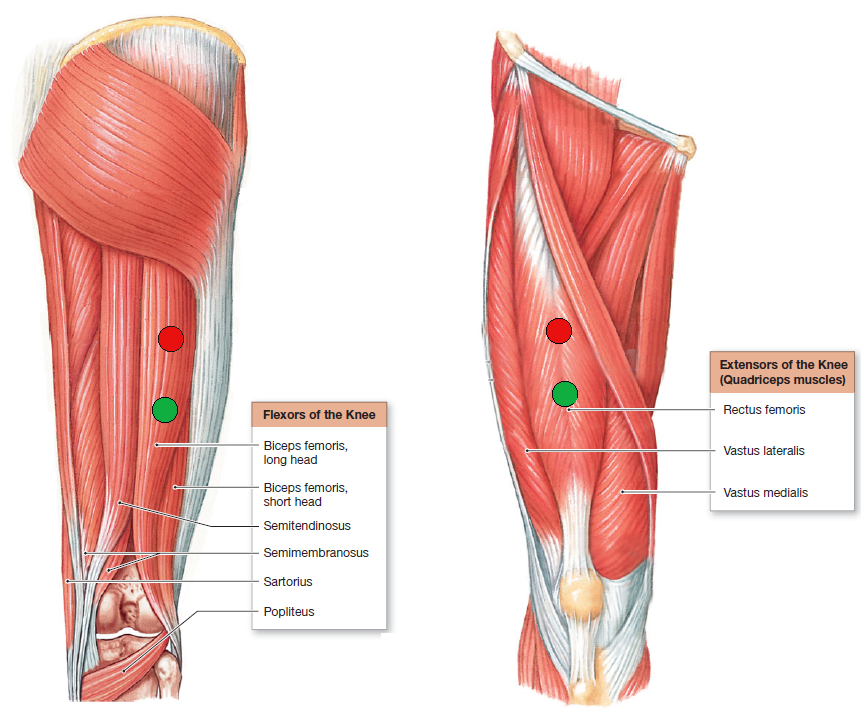
\includegraphics[width=0.5\textwidth]{figures/laarmuskler.png}
\caption{Låret set anteriot og posteriot. Placering af positiv (rød) samt negativ (grøn) elektroder ses på biceps femoris og rectus femoris \citep{martini2012}.}
\label{fig:laarmuskler}
\end{figure}

Den fælles referenceelektrode placeres, ligeledes efter Seniam's anvisninger, omkring anklen \citep{seniam2016}. Placeringen af reference elektroden ses af \autoref{fig:reference}.

\begin{figure}[H]
\centering
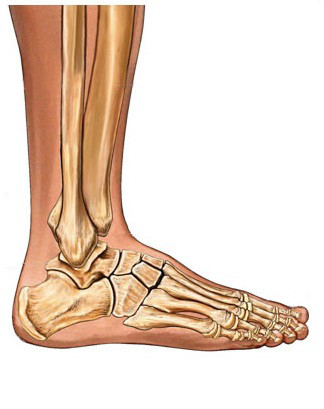
\includegraphics[width=0.3\textwidth]{figures/reference}
\caption{Placering af den fælles referenceelektrode omkring anklen \citep{ankle2016}.}
\label{fig:reference}
\end{figure}

Til forsøget benyttes endvidere to accelerometre, som måler i y-aksen. Disse benyttes for at kunne identificere vinklen af knæet under øvelsen. For så vidt muligt at kunne stabilisere accelerometrene under udførelsen af forsøget, placeres disse på breadboards. 
Som det fremgår af \autoref{fig:accelerometervinkel} placeres det ene accelerometer midt på den laterale side af låret, parallelt med femur. Det andet accelerometer placeres midt på den laterale side af underbenet, parallelt med tibia. Knæets vinkel i oprejst position måler 180$^{\circ}$, hvilket svarer til en 0 g-påvirkning. Vinklen af knæet ændres i takt med udførelse af en squat-øvelse, hvorved g-påvirkningen bevæger sig mod 1. Den samlede vinkel af knæet bestemmes ud fra de to accelerometres parametre. Udregningen for dette kan ses i \autoref{sec:test_acc}.

\begin{figure}[H]
\centering
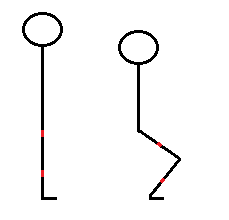
\includegraphics[width=0.4\textwidth]{figures/accelerometervinkel.png}
\caption{Placering af referenceelektroderne omkring anklen \citep{ankle2016}.}
\label{fig:accelerometervinkel}
\end{figure}

Til identificering af støj fra EMG-forstærkeren fortages der baselinemålinger, som senere analyseres via en frekvensanalyse. Det samme gør sig gældende for identificeringen af EMG-signalets frekvensområde. Dette vil foregå under udførelsen af en squat-øvelse.
En squat-øvelse defineres, således den kan gengives på tværs af forsøgspersonerne.\vspace{3mm}
\begin{enumerate}
\item Forsøgspersonen står i oprejst position. Fødderne placeres med en afstand svarende til ens skulderbredde, hvortil tåspidserne peges let til siderne
\item Hofte og knæ bøjes således kroppen sænkes kontrolleret. Dette fortsættes indtil en vinkel på 90$^{\circ}$ af knæet er opnået
	\begin{itemize}
	\item Ryggen holdes ret under squat-øvelsen 
	\item Knæene må ikke gå ud over tåspidserne 
	\end{itemize}
\item Kroppen returneres til udgangspunksposition
\end{enumerate} \vspace{3mm}
En illustration af squat-øvelsen ses af \autoref{fig:squat}
En nedadgående squat-øvelse defineres som punkt $1-2$ i overstående, hertil forbliver forsøgspersonen i en siddende squat indtil den givene måling er gennemført.

\begin{figure}[H]
\centering
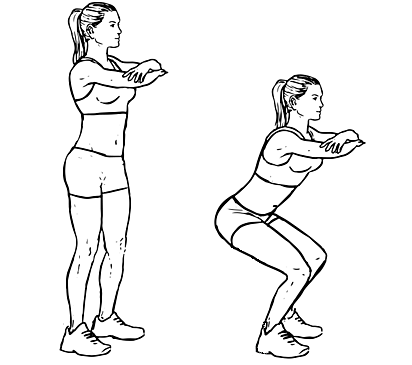
\includegraphics[width=0.5\textwidth]{figures/squat.png}
\caption{Squat-øvelse \citep{squat2015}.}
\label{fig:squat}
\end{figure}


Da mikrokontrolleren benytter en operationsspænding på $XX~V$ ønskes en signalamplitude under operationsspændingen, da dette vil bidrage til en mindre støjpåvirkning. 
%Noget angående signal to noise ratio 

%For at simulere den påvirkning som accelerometeret udsættes for og derved identificere det maksimale og minimale outputsignal roteres accelerometeret i en langsom rotation fra $0 - 90^{\circ}$ både til højre og venstre. Herudover måles accelerometerets påvirkning i henholdsvis 0 og 1 g-påvirkning for at identificere accelerometeres påvirkning samt, hvorvidt dette stemmer overens med databladet.


\subsection{Forsøgsopstilling}
Forsøgsopstillingen opstilles, hvoraf EMG-forstærker samt accelerometrene anvendes. 

\begin{itemize}
\item Identificering af musklerne rectus femoris og biceps femoris 
\item Huden prepereres ved fjernelse af hår og døde hudceller samt desinficering 
\item Elektroderne påsættes
	\begin{itemize}
	\item Elektrodesæt 1: positiv og negativ på rectus femoris
	\item Elektrodesæt 2: positiv og negativ på biceps femoris
	\item Fælles reference på anklen
	\end{itemize} 
\item Accelerometrene placeres 
	\begin{itemize}
	\item Accelerometer 1: midt på den laterale side af låret, parallelt med femur
	\item Accelerometer 2: midt på den laterale side af underbenet, parallelt med tibia 
	\end{itemize}
\item Accelerometrene vælges til at måle i y-aksen
\end{itemize}

\subsection{Fremgangsmåde}
Forsøgspersonen placeres på et fast punkt under forsøget. Øvelserne udføres tre gange, hvoraf der ud fra målingerne foretages en senere databehandling. 

\subsubsection{Pilotforsøg}
\textbf{Baseline måling}
\begin{itemize}
\item 10 sekunders måling, hvor forsøgspersonen står oprejst
\end{itemize}

\textbf{1. måling}
\begin{itemize}
\item Måling i en nedadgående squat-øvelse
	\begin{itemize}
	\item 1 sekunds baseline oprejst
	\item 4 sekunder nedadgående squat 
	\item 1 sekunds baseline i squat-øvelsen
	\end{itemize}
\end{itemize}
	
\textbf{2. måling}
\begin{itemize}
\item Måling i en squat-øvelse
	\begin{itemize}
	\item 1 sekunds baseline oprejst
	\item 4 sekunder nedadgående squat 
	\item 4 sekunder opadgående squat
	\item 1 sekunds baseline oprejst
	\end{itemize}
\end{itemize}

%\subsubsection{Accelerometer}
%\begin{itemize}
%\item 10 sekunders baseline måling i 0 g-påvirkning (0$^{\circ}$)
%\item 10 sekunders baseline måling i 1 g-påvirkning (90$^{\circ}$)
%\item 10 sekunders måling ved rotation fra $0-1$ g-påvirkning både til højre og venstre
%	\begin{itemize}
%	\item 1 sekunds baseline måling i 0 g-påvirkning (0$^{\circ}$
%	\item 8 sekunders rotation mod 1 g-påvirkning (90$^{\circ}$)
%	\item 1 sekunds baseline måling i 1 g-påvirkning (90$^{\circ}$)
%	\end{itemize}
%\end{itemize}

